\documentclass[a4j, twocolumn]{article}

%% プリアンブル部 %%
\usepackage{fancybox}
\usepackage{ascmac}
\usepackage[dvipdfmx]{graphicx}
\usepackage{amsmath}
\usepackage{pgffor}
\usepackage{ulem}
\usepackage{booktabs} % 表を綺麗にするため

\begin{document}

\title{記号創発の構造的アプローチ}
\author{高久　欣也 \thanks{MEKOU}}
\date{\today{}}

\maketitle

\section{はじめに}
私の趣味はプログラミングと言っていいだろう。計算してみると、約1万時間もの時間をプログラミングに費やしていることになる。卒業研究において、自ら持ち込んだテーマを追求できるのは、エンジニアとして非常に幸運なことだと感じている。本稿では、現在取り組んでいる研究の核心について紹介する。

\section{研究テーマについて}
\subsection{背景}
私は介護ロボットの実用化に強い関心がある。その一環として、LLM（大規模言語モデル）のような「知能」をロボットに搭載できないかと考えた。

しかし、現状のLLMはロボティクスにおいて「不完全」であると断言せざるを得ない。既存のAIは高次元空間上の確率分布を近似しているに過ぎず、Transformer主導の構造には物理世界との接地（シンボル・グラウンディング）において致命的な限界があるからだ。
「赤」という情報をテキストとしていくら学習しても、物理的な「赤」を認識することはできない。ロボティクスに必要なのは、統計的な相関ではなく、物理的制約に基づいた信頼性と安定性である。

本研究では、認知工学の知見を取り入れつつ、Attentionや重み共有といった近代的な技術を「構造的アプローチ」によって再定義し、Rust/wgpuによる自作エンジンで実装を試みている。

\section{思想的背景}
知性というものを、ある種の「構造的必然」として捉える。
認知工学的には、言語の意味は記号単体ではなく、相対的な関係性によって設定される。子供の成長過程を考えると教師データをもとに記号を習得するわけではない。
記号創発とは、外部環境（社会や物理的フィードバック）との相互作用によって生まれる「歪みの補正プロセス」であると考えることができる。

\section{研究内容について}
実装の具体例として、以下の問いを立てる。
\begin{screen}
\textbf{LLMの出力とマルチモダリティな感覚情報の統合を、行列演算における競合解消として記述できないか。}
\end{screen}
これにより、ロボットの自立性と情報の整合性を定量的に検証することが可能になる。

\section{実装状況}
現在の開発フェーズは以下の通りである。
\begin{itemize}
    \item \textbf{TODO}
    \begin{itemize}
        \item XOR問題によるパーセプトロンの基本テスト（完了）
        \item GPUメモリ配線およびシェーダーによるLLMパイプラインの実装（難航中）
        \item モダリティ統合テスト（進行中）
    \end{itemize}
    \item \textbf{任意目標}
    \begin{itemize}
        \item 介護実習の知見を活かしたロボティクスによる実演
    \end{itemize}
\end{itemize}

\section{独自性と技術スタック}
最大のこだわりは、Pythonをシステムから排除し、Rust、wgpu、独自シェーダーでGPU実装を行っている点である。
既存ライブラリでは、ネットワークの「動的な構造変更」が困難であったため、車輪の再開発を承知で自前実装に至った。
特に、NNが局所解に陥った際、次元を動的に拡張して解決を図る手法は、幾何学的なアプローチをとる本研究のユニークな点である。

\section{技術的説明}
\subsection{使用技術}
wgpuを用い、グラフィックス用の計算資源を汎用計算（GPGPU）に転用している。リダクション演算を最適化することで、CPU単一スレッド比で数十倍から百倍以上の計算速度を期待できる。

\subsection{アプローチの比較}
既存の統計的アプローチと、本研究の構造的アプローチの差異を以下にまとめる。

\begin{table}[h]
\centering
\caption{アプローチの対比}
\begin{tabular}{l|l|l}
\toprule
項目 & 統計的アプローチ & 構造的アプローチ \\ \midrule
学習原理 & 出現確率の近似 & 幾何学的拘束 \\
構造 & 固定（静的） & 次元拡張（動的） \\
接地 & シンボル未接地 & 物理的整合性 \\ \bottomrule

\end{tabular}
\end{table}

\subsection{数理的解釈と次元拡張アルゴリズム}
NNの基本素子は、以下の線形変換と非線形活性化関数 $\sigma$ で記述される。
\begin{equation}
    y = \sigma\left(\sum_{n=1}^N w_n x_n + b\right)
\end{equation}
これは$N$次元空間を超平面で分割する操作を意味する(次章にて説明)。従来のAIはこの$N$（次元数）を固定して学習を行うが、データが非線形に混在する局所解では、分割不能な状態に陥る。

本研究の「次元拡張アルゴリズム」は、誤差 $\delta \text{loss}$ の改善が停滞した際、動的に $N \to N+1$ への拡張を行い、新たな次元からの射影によって線形分離を可能にする。シェーダーレベルでのコンパイルのため、この構造変化は極めて高速に実行される。

\subsection{NNへの補足説明}
例えばXORでは対照にクラスが分布されているので、直線による分類が不可能。なので、ネットワークの深さを増し、非線形変換を繰り返し、境界線を曲線化すれば良い。曲線としてはこのような曲線を描く必要がある(図~\ref{fig:ref1})。
XORの場合は曲線つまり、深さを増やし、適切に学習が進まればいいが、問題はクラスの周りをクラスが囲っているときである。これには次元を増やして取ればいい。３次元でも周りを囲っているなら、４次元から取ってあげればいい。
この、クラスの周りを別クラスが囲って、包囲しているとき境界を取るのが難しい、こういったときLOSSが下がらなくなるそうなれば次元をあげて解きやすくしてやれば良いと言うのが基本の考えである。

\begin{figure}[htbp]
    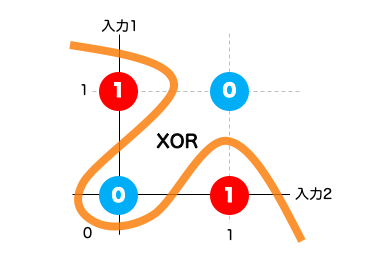
\includegraphics[width=0.8\columnwidth]{xor.png}
    \label{fig:ref1}
    \caption{XOR問題でのNN}
\end{figure}

\subsection{感情行列によるデバッグ}
記号接地の検証として「感情行列」を導入する。ロボットが「重い」と発話しつつ、実際のトルクセンサーが低負荷を示した場合、この行列内に競合（不一致）が発生する。この矛盾を検知・解消するプロセスこそが、実世界への接地を意味する。

\subsection{技術のまとめ}
本研究で提案する構造的アプローチは、記号を確率的なトークンとしてではなく、物理センサーと同期した「幾何学的な拘束条件」として扱う。これにより、ロボットが発する言葉の一つ一つに、物理的な実体（トルク、重心、接触圧など）を伴わせることが可能となる。これは、単なる対話エンジンとしてのAIではなく、人間の身体を補助する「生命模倣の知能」へのマイルストーンである。

\section{研究過程で見つかった知見}
\begin{description}
    \item [NN構造への知見] 本末転倒に聞こえるかもしれないが、要するにNN自体、行列計算と考えると、コード（目標関数）と１対１の動作を行うことに加え、モジュールとして扱えれると言う考えである。anthropicなどがこの辺の研究をしている。MCPなどがその例でLLMが意味理解をできていないから外のツールを頼っているが、私はこの仕組みの脆弱性を問いたい。
    \item [境界探索問題としての認知] 認知とは「自己と他者の境界」を定義するプロセスではないか。まず、NN自体が人間のシナプス活性の模倣であること、それの模倣のレイヤーなどの有効性も指摘されている。加えて、私はあくまで、このために感情行列を作ったが、人間も同じような仕組みで動いているのではないだろうか。
    \item [脳のハッキング可能性] 人間の脳は他者との境界概念が意外にも脆弱である。幻覚痛などの現象は、脳内の整合性行列が外部刺激で上書き可能であることを示唆している。この知見は、義手と人間のギャップを埋める技術に応用できる可能性がある。
\end{description}

\section{考察：介護現場における実用シナリオ}
本研究の「構造的アプローチ」が真価を発揮するのは、抽象的な概念が具体的な身体感覚と矛盾した際である。介護現場における実用シナリオを想定し、その優位性を考察する。

\subsection{感覚矛盾の検知と解消}
例えば、ロボットが被介護者を持ち上げる際、視覚センサー（被介護者の表情や姿勢）から得られた「安心」というラベルと、触覚センサー（筋電位や抵抗値）から得られた「過度な緊張」というラベルが同時に存在する場合を考える。
従来の統計的LLMでは、学習データの頻度に従っていずれか一方を「もっともらしい出力」として採択する傾向があるが、これは介護現場において重大な事故に繋がりかねない。

\section{展望}
この研究の後の話としては、ロボティクスが最終目標である。SFに感化されているだけである。結局研究とか関係なく、AIが身体を獲得するのが人間最後の発明と考えてもいいだろう。
私はそれを作り、介護施設を始め、ブルーカラーに導入し、社会構造をアップデートして、できれば、巨額の資金を稼ぎたいのだ。
そのために、SFレベルのロボットを逆算し、要件定義して作ってしまえばいいだろうと思い日々勤しんでいるわけです。
高専５年間の集大成だなと思います。個人の分散処理から、低レイヤー、NNの自作がいきています。
ただ、現在はLLMでなかなか思うように学習せず苦しんでおります。

\section{まとめ}
本研究は、幾何学的な視点からNNを再定義し、自発的な記号創発を目指すものである。生命の定義といった形而上学的議論ではなく、あくまで「人間とデジタルのインターフェース統合」という工学的解決を目的としている。

\begin{thebibliography}{9}
\bibitem{ref1} 谷口忠大『記号創発ロボティクス』講談社
\bibitem{ref2} 斎藤康毅『ゼロからつくるDeep Learning』オライリー・ジャパン
\end{thebibliography}

\end{document}